% Chapitre 11 -- ED-20 : le réseau triangulaire n'est pas un minimum local de l'énergie de point zéro pour exp(-pi r^2)
% Sources : results/discovery_journal_2026/TOP20.json (pick 11), papers/p2_certified_zero_point/{main.tex,AUDIT.md,REVISION.md,publication_meta.json,data/},
% papers/p3_zero_point_physical/data/leanchecker_replay.json (rejeu du module Lean). Figure : code/fig11.py.
\chapter{Parfait au repos, pas quand il frissonne}

\reference{Publié le 26 octobre 2026. doi:10.5281/zenodo.23655392}

\section*{L'idée en une image}

Imaginez des billes qui se repoussent, posées sur une table. Laissées tranquilles, elles
s'arrangent en triangles : chaque bille a six voisines, comme les cellules d'une ruche. Pour
la force étudiée ici, une répulsion en forme de cloche (elle vaut $e^{-\pi r^2}$ à la distance
$r$), cet arrangement triangulaire est le meilleur des réseaux réguliers quand les billes sont
immobiles : c'est un résultat ancien de la littérature, que ce travail cite de seconde main et ne revérifie pas.

Mais en physique quantique, rien n'est jamais tout à fait immobile. Même au zéro absolu, chaque
particule frissonne un peu, et ce frisson coûte une énergie dite \og de point zéro\fg{}. La
question, notée QU-1 dans le projet, était naturelle : le réseau qui gagne au repos gagne-t-il
aussi quand on compte ce frisson ? Un calcul approché antérieur (au crayon, au sens du
niveau~X) disait déjà non. Ce chapitre raconte comment ce \og non\fg{} a été rendu certain, sur
un morceau précis de la question.

\begin{analogie}
On croyait la bille posée au fond d'une cuvette. On la pousse d'un cheveu, dans une direction
bien choisie, et l'on constate que l'altitude baisse : ce n'était donc pas le fond.
\emph{Où l'image s'arrête :} ici rien ne roule ; on compare les énergies de deux arrangements
figés, très proches l'un de l'autre. Et l'on ne sait pas, par ce résultat seul, si l'on était
au sommet d'une bosse ou sur un col : on sait seulement que ce n'était pas le fond.
\end{analogie}

\section*{Ce qui a été fait}

On part du réseau triangulaire et on le déforme d'une quantité $t$ par un léger cisaillement
qui garde la même surface par bille. On note $E(t)$ l'énergie de point zéro par bille. Le
travail montre que $E(t)<E(0)$ pour tout $t$ non nul tel que $|t|\le 10^{-5}$.

L'énergie $E(t)$ est une moyenne de racines carrées de matrices, très difficile à encadrer
directement. L'astuce consiste à construire un \emph{toit} $U(t)$ : une fonction toujours
au-dessus de $E$, qui la touche exactement en $t=0$. Si le toit redescend des deux côtés de
$0$, le terrain dessous redescend aussi. Pour cela, il suffit de prouver que la courbure du
toit reste négative sur toute la petite fenêtre ; le calcul certifié la borne par $-1{,}84156$.
Alors $E(t)-E(0)\le -0{,}92\,t^2$ : à $t=10^{-5}$, une baisse d'au moins
$9\times10^{-11}$ en unités du calcul. C'est minuscule, mais c'est un signe certain.

\begin{encadre}
\textbf{À faire avec un crayon : pourquoi le toit est au-dessus.} Prenez un nombre $d$ et une estimation $x$
de sa racine. Comme $(\sqrt d - x)^2\ge 0$, on a toujours
\[\sqrt d\;\le\;\tfrac12\Bigl(x+\frac{d}{x}\Bigr),\]
avec égalité quand $x=\sqrt d$. Essayez $d=10$, $x=3$ : le membre de droite vaut
$\tfrac12(3+\tfrac{10}{3})=\tfrac{19}{6}\approx3{,}1667$, et $\sqrt{10}\approx3{,}1623$ est
bien en dessous. Le travail utilise la même inégalité pour des matrices $2\times2$.

\textbf{À faire avec un crayon : le signe final.} Les trois nombres certifiés, arrondis ici
contre nous (vers le côté qui rapproche de zéro), sont $-1{,}900167$, $1{,}833534$ et
$0{,}031965$. La borne vaut au plus
$-1{,}900167+1{,}833534\times0{,}031965\approx-1{,}900167+0{,}058609=-1{,}841558$,
négative. Le programme Lean refait ce calcul avec les fractions exactes.
\end{encadre}

\section*{Comment on s'est assuré que ce n'est pas faux}

La chaîne a trois maillons, et ils n'ont pas le même niveau.
\niveau{A} \emph{Le juge a regardé} pour la logique et l'arithmétique : l'inégalité des matrices $2\times2$, le
raisonnement \og toit qui descend, donc terrain qui descend\fg{} et le signe des fractions sont
vérifiés pas à pas par le noyau de Lean, le petit programme juge des preuves. Les axiomes
restent dans la liste courte autorisée, et un rejeu du module par le noyau est passé.
\niveau{C} pour les intégrales, au sens où personne ne les a vérifiées à la machine : elles sont encadrées par de l'arithmétique d'intervalles
rigoureuse (206\,468 cellules, aucune en échec), exécutée par un programme mais non relue par
le juge. \niveau{C} aussi pour la \og colle\fg{} : un raisonnement, ici mené par des agents
d'IA et non par un humain, que ni machine ni personne n'a vérifié. Le résultat d'ensemble est donc de niveau~C, et
le papier le dit.

Les contrôles ont joué leur rôle. Pour une cloche plus étroite ($e^{-2\pi r^2}$), le réseau
triangulaire \emph{est} un minimum local selon le calcul approché : la même méthode doit alors
échouer, et elle échoue (la borne reste positive, vers $+12{,}8$), et le juge refuse le
certificat. Une fausse preuve plantée exprès est démasquée par la liste des axiomes. Un agent
auditeur distinct a refait le calcul avec des cellules 8 à 25 fois plus larges : le signe
reste négatif. Il a aussi recodé les quantités autrement, en virgule flottante, et trouvé des
valeurs à l'intérieur des encadrements. Son verdict, \og accepter avec corrections\fg{},
demandait deux corrections de texte, dont une phrase mathématique fausse ; elles sont
appliquées. Aucun humain n'a relu ce travail.

\section*{Ce que ça ne dit pas}

\begin{limite}
\begin{itemize}
\item Un seul chemin de déformation, une fenêtre de $10^{-5}$, une seule force, des réseaux
  réguliers en deux dimensions, et l'approximation \og harmonique\fg{} des vibrations.
\item Le résultat est à sens unique : la méthode peut dire \og pas un minimum\fg{}, jamais
  \og minimum\fg{}. Elle borne une courbure par le haut, sans l'encadrer des deux côtés.
\item L'objectif annoncé à l'avance (une courbure certifiée des deux côtés) n'est pas
  atteint ; le papier le signale comme un écart au préenregistrement.
\item Le même certificat marche pour $e^{-\pi r^2/2}$, mais ce cas n'était pas prévu : c'est
  un sous-produit, pas un test.
\item Rien n'est dit du meilleur réseau pour l'énergie de point zéro, ni du cristal quantique
  complet.
\end{itemize}
\end{limite}

C'est pourtant une leçon utile : \og le meilleur au repos\fg{} et \og le meilleur en
frissonnant\fg{} ne coïncident pas, et on le sait maintenant au-delà du calcul approché.

\section*{Pour aller plus loin}

Le papier (8 pages, en anglais) donne la démonstration étape par étape, à côté des énoncés
Lean correspondants : doi:10.5281/\allowbreak zenodo.23655392. La même question, pour des forces plus
physiques, est reprise dans doi:10.5281/\allowbreak zenodo.23663551.

\begin{figure}[ht]
\centering
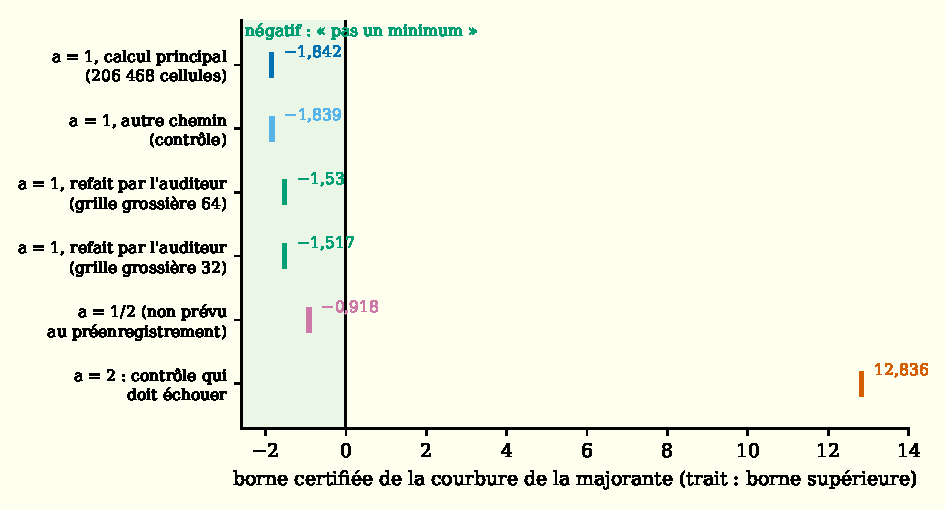
\includegraphics[width=\linewidth]{figures/c11_courbures}
\caption{Bornes certifiées de courbure : négatives pour $a=1$ (calcul, contrôle, reprises de l'auditeur) et $a=1/2$, positive pour le contrôle $a=2$.}
\end{figure}
